\section{Background}


\section{AR Libraries}


\section{Software Architecture}
In order to identify platforms that are good for implementing AR on smart- phones, prototyping was divided into three platforms to explore them such as Vuforia (Unity/Android), ARKit(iOS) and AR Core (Android). Building test applications to discover how they assist with implementation in our application and what problem will be faced during the implement.

\subsection{Vuforia (Unity/Android)}
Unity is a cross-platform game engine, used to test a simple AR camera prototype where the device’s camera hovers an image, and displays information about that image on the device (Figure~\ref{fig:vulforia}). The application was built using Vuforia, an SDK that enables recognition, and tracking of image targets. This library can be used for the exploration case in the use case model. Although, there is a lack of tools for locating user current location compared to Android.


\subsection{ARKit (iOS)}
A similar prototype to Unity (Figure~\ref{fig:ARKit}) was built on Apple’s ARKit using Swift [8], which was easy to learn. It was intuitive to implement AR features as there was detailed documentation, but logging GPS data was harder compared to Android therefore we would not able to work with ARKit.


\subsection{AR Core (Android)}
ARCore was used to create a simple 3D model showing on a mobile device when its camera targeted flat surface (Figure~\ref{fig:ARCore}). Compared to iOS, it is easier to log GPS location, although connecting the user interface to the scripts was more challenging.

After exploring this three prototype, we found ARCore(Android) will work best in our AR application. ARCore helps us to identify the user current GPS location therefore our Developer team need to put lot of effort into delivering a right location on user’s screen.

\subsection{Test Example}
\subsubsection{Vuforia}
\begin{figure}[H]
\centering  
\begin{tabular}{cc}
  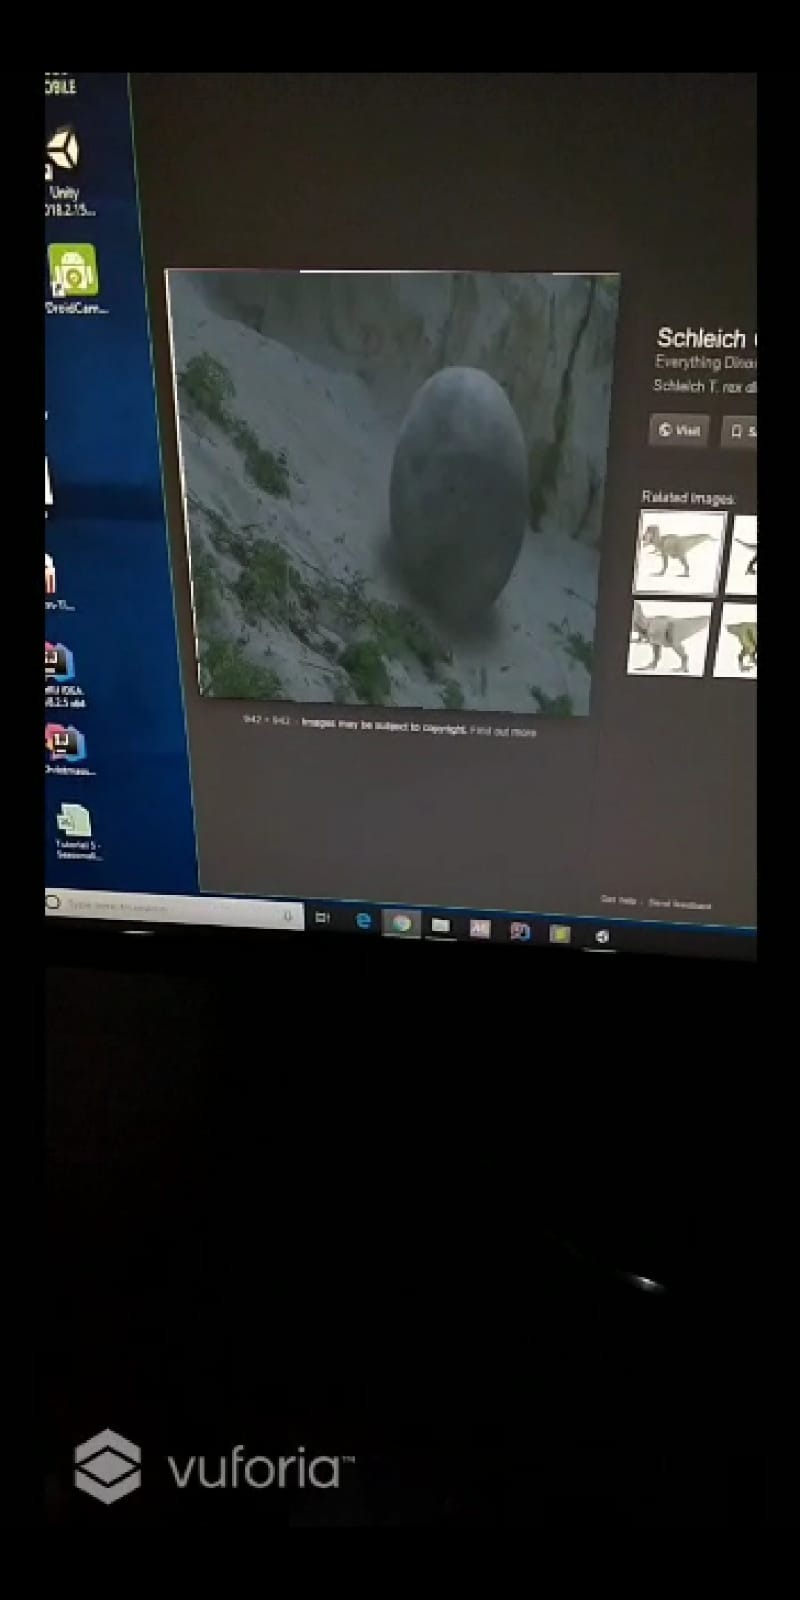
\includegraphics[width=60mm, height=100mm]{prototypes/ar/vulforia/1.jpeg} &   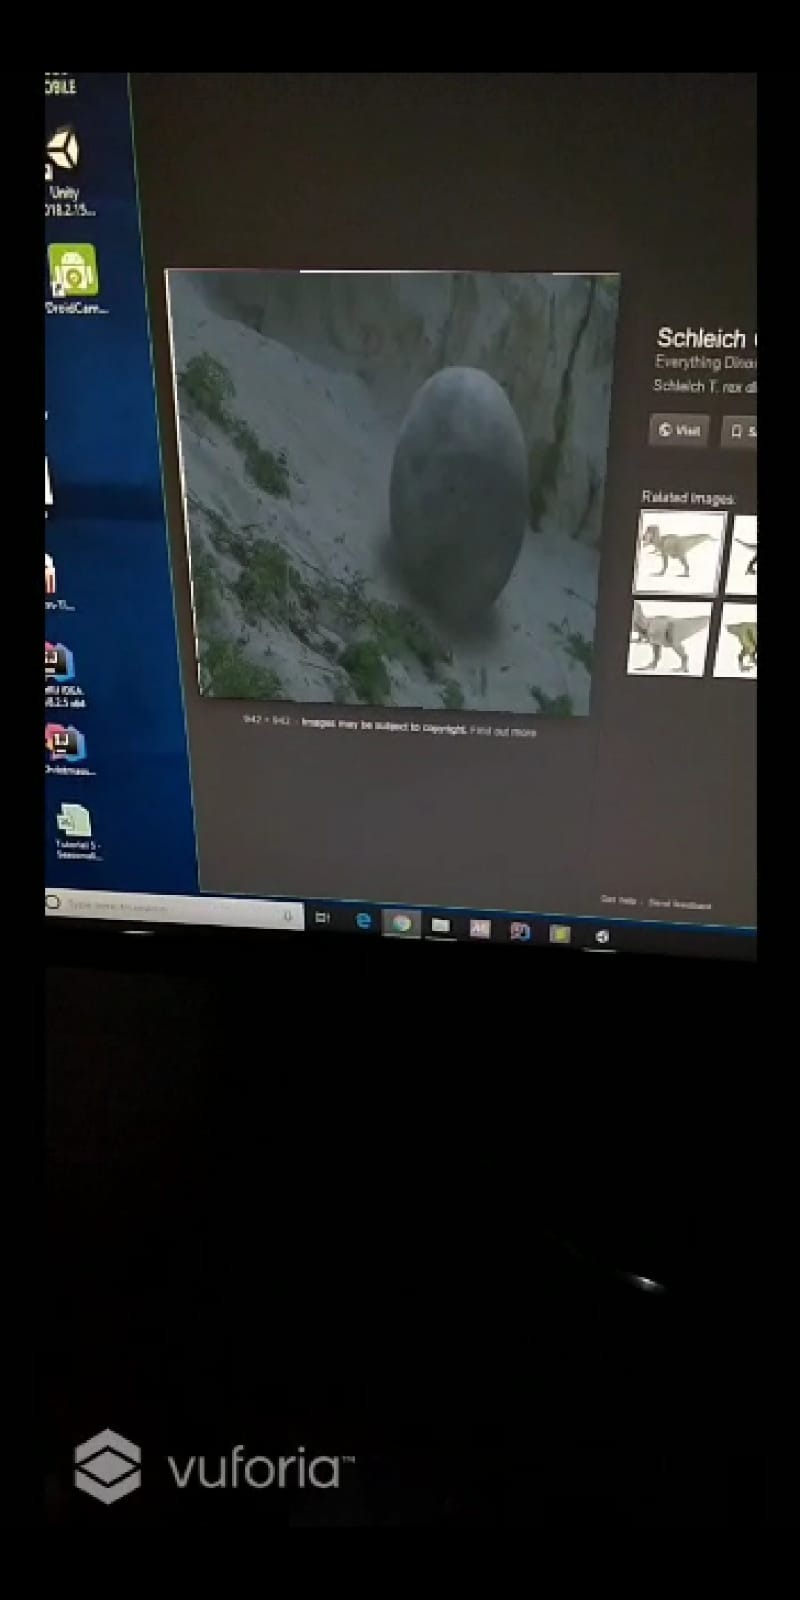
\includegraphics[width=60mm, height=100mm]{prototypes/ar/vulforia/2.jpeg} \\
(a) Camera over image & (b) Video superimposed on top of image\\[6pt]
\end{tabular}
\caption{Vuforia prototyping on Android device}
\label{fig:vulforia}
\end{figure}


\newpage
\subsubsection{ARKit}
\begin{figure}[H]
\centering  
\begin{tabular}{cc}
  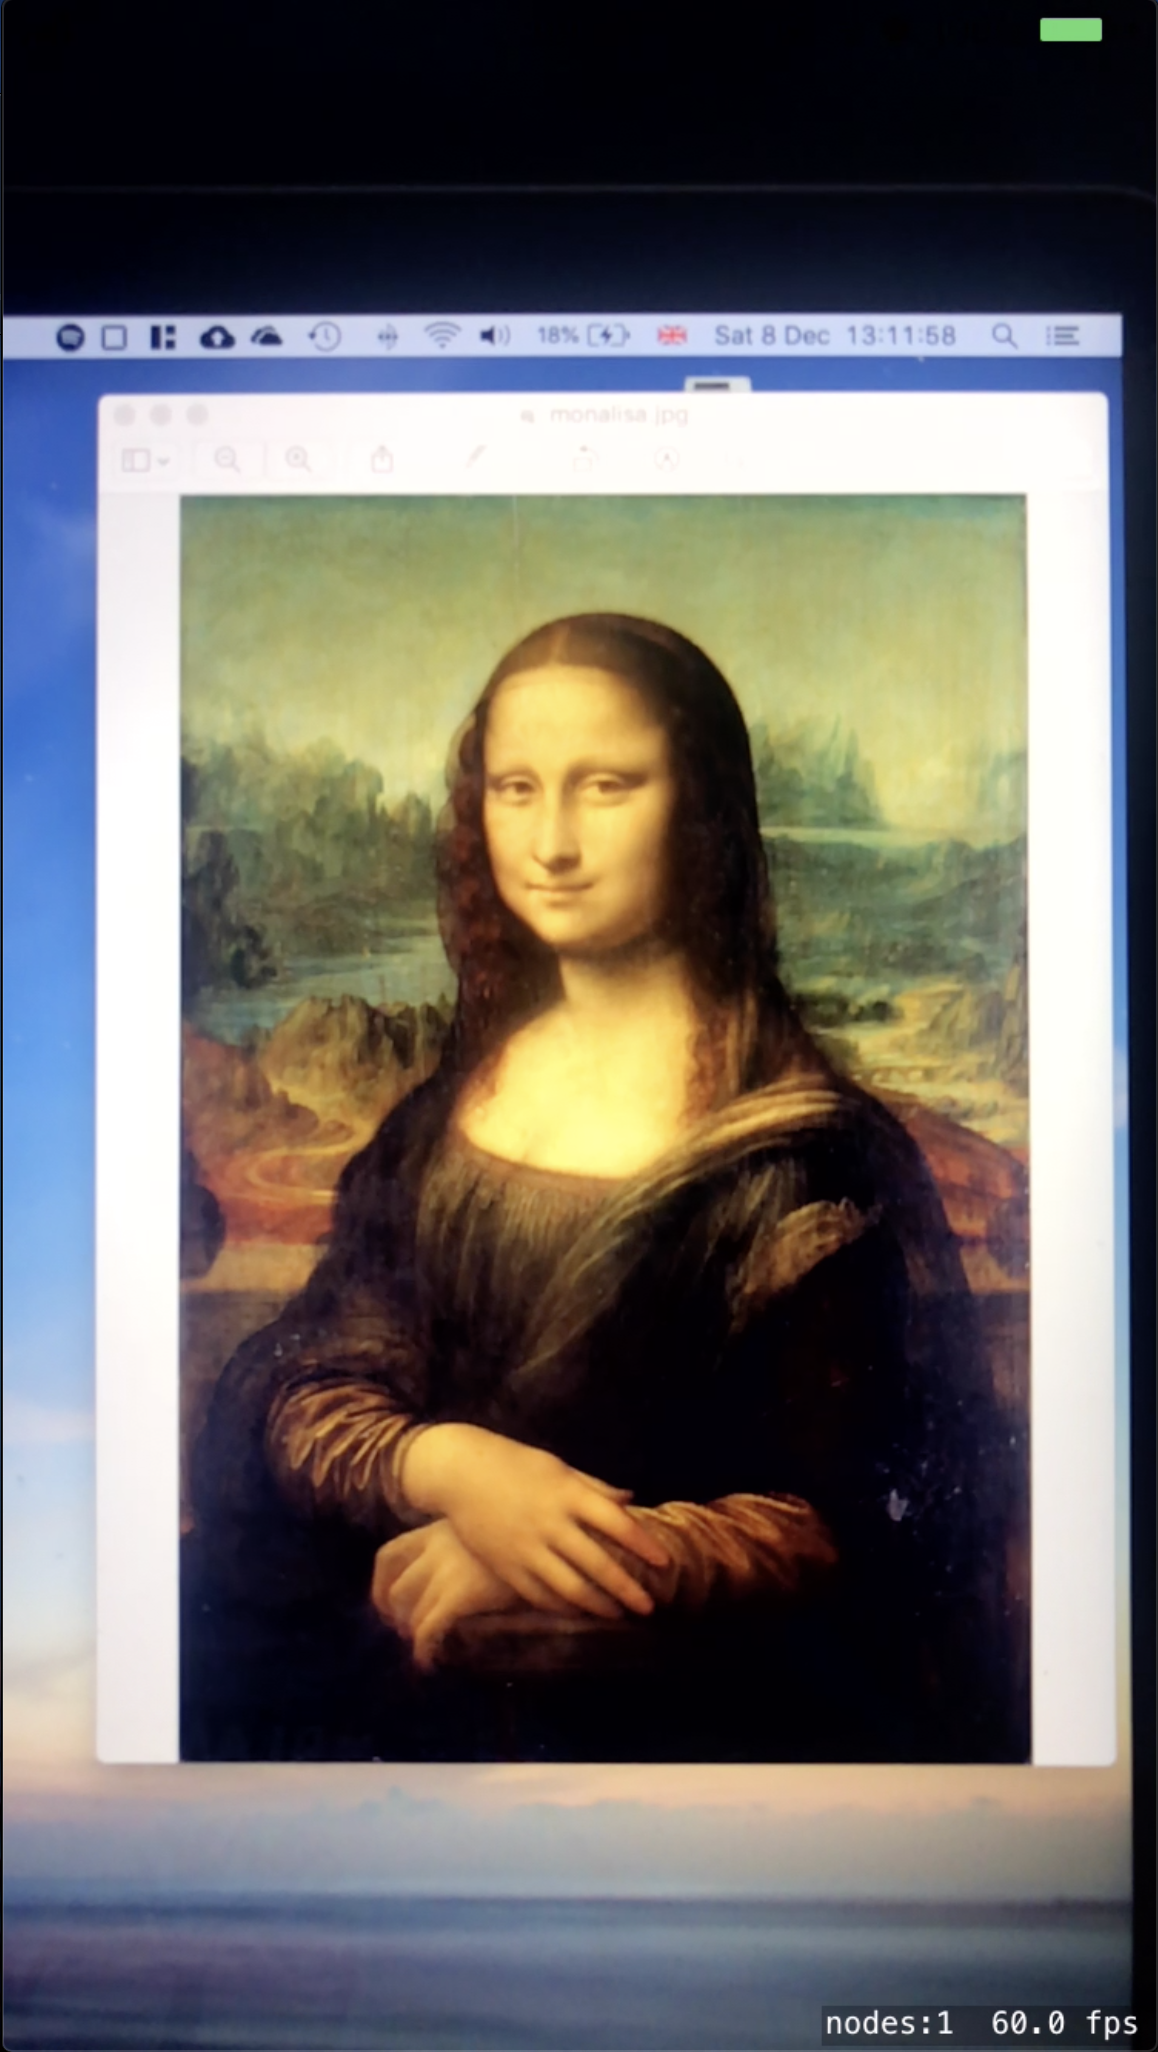
\includegraphics[width=60mm, height=100mm]{prototypes/ar/ios/1.png} &   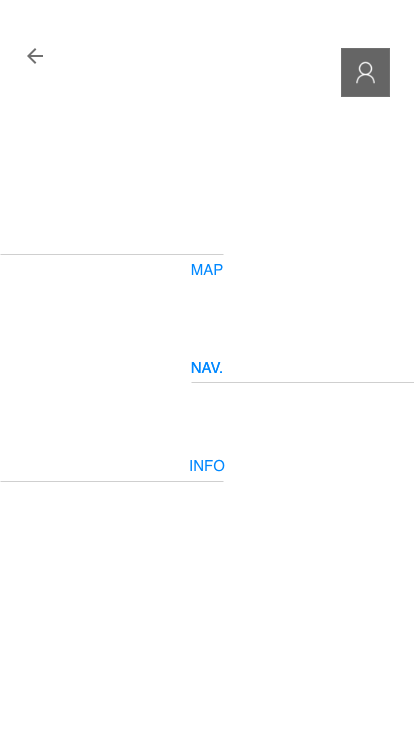
\includegraphics[width=60mm, height=100mm]{prototypes/ar/ios/2.png} \\
(a) Camera over image & (b) Image recognised and displaying information \\[6pt]
\multicolumn{2}{c}{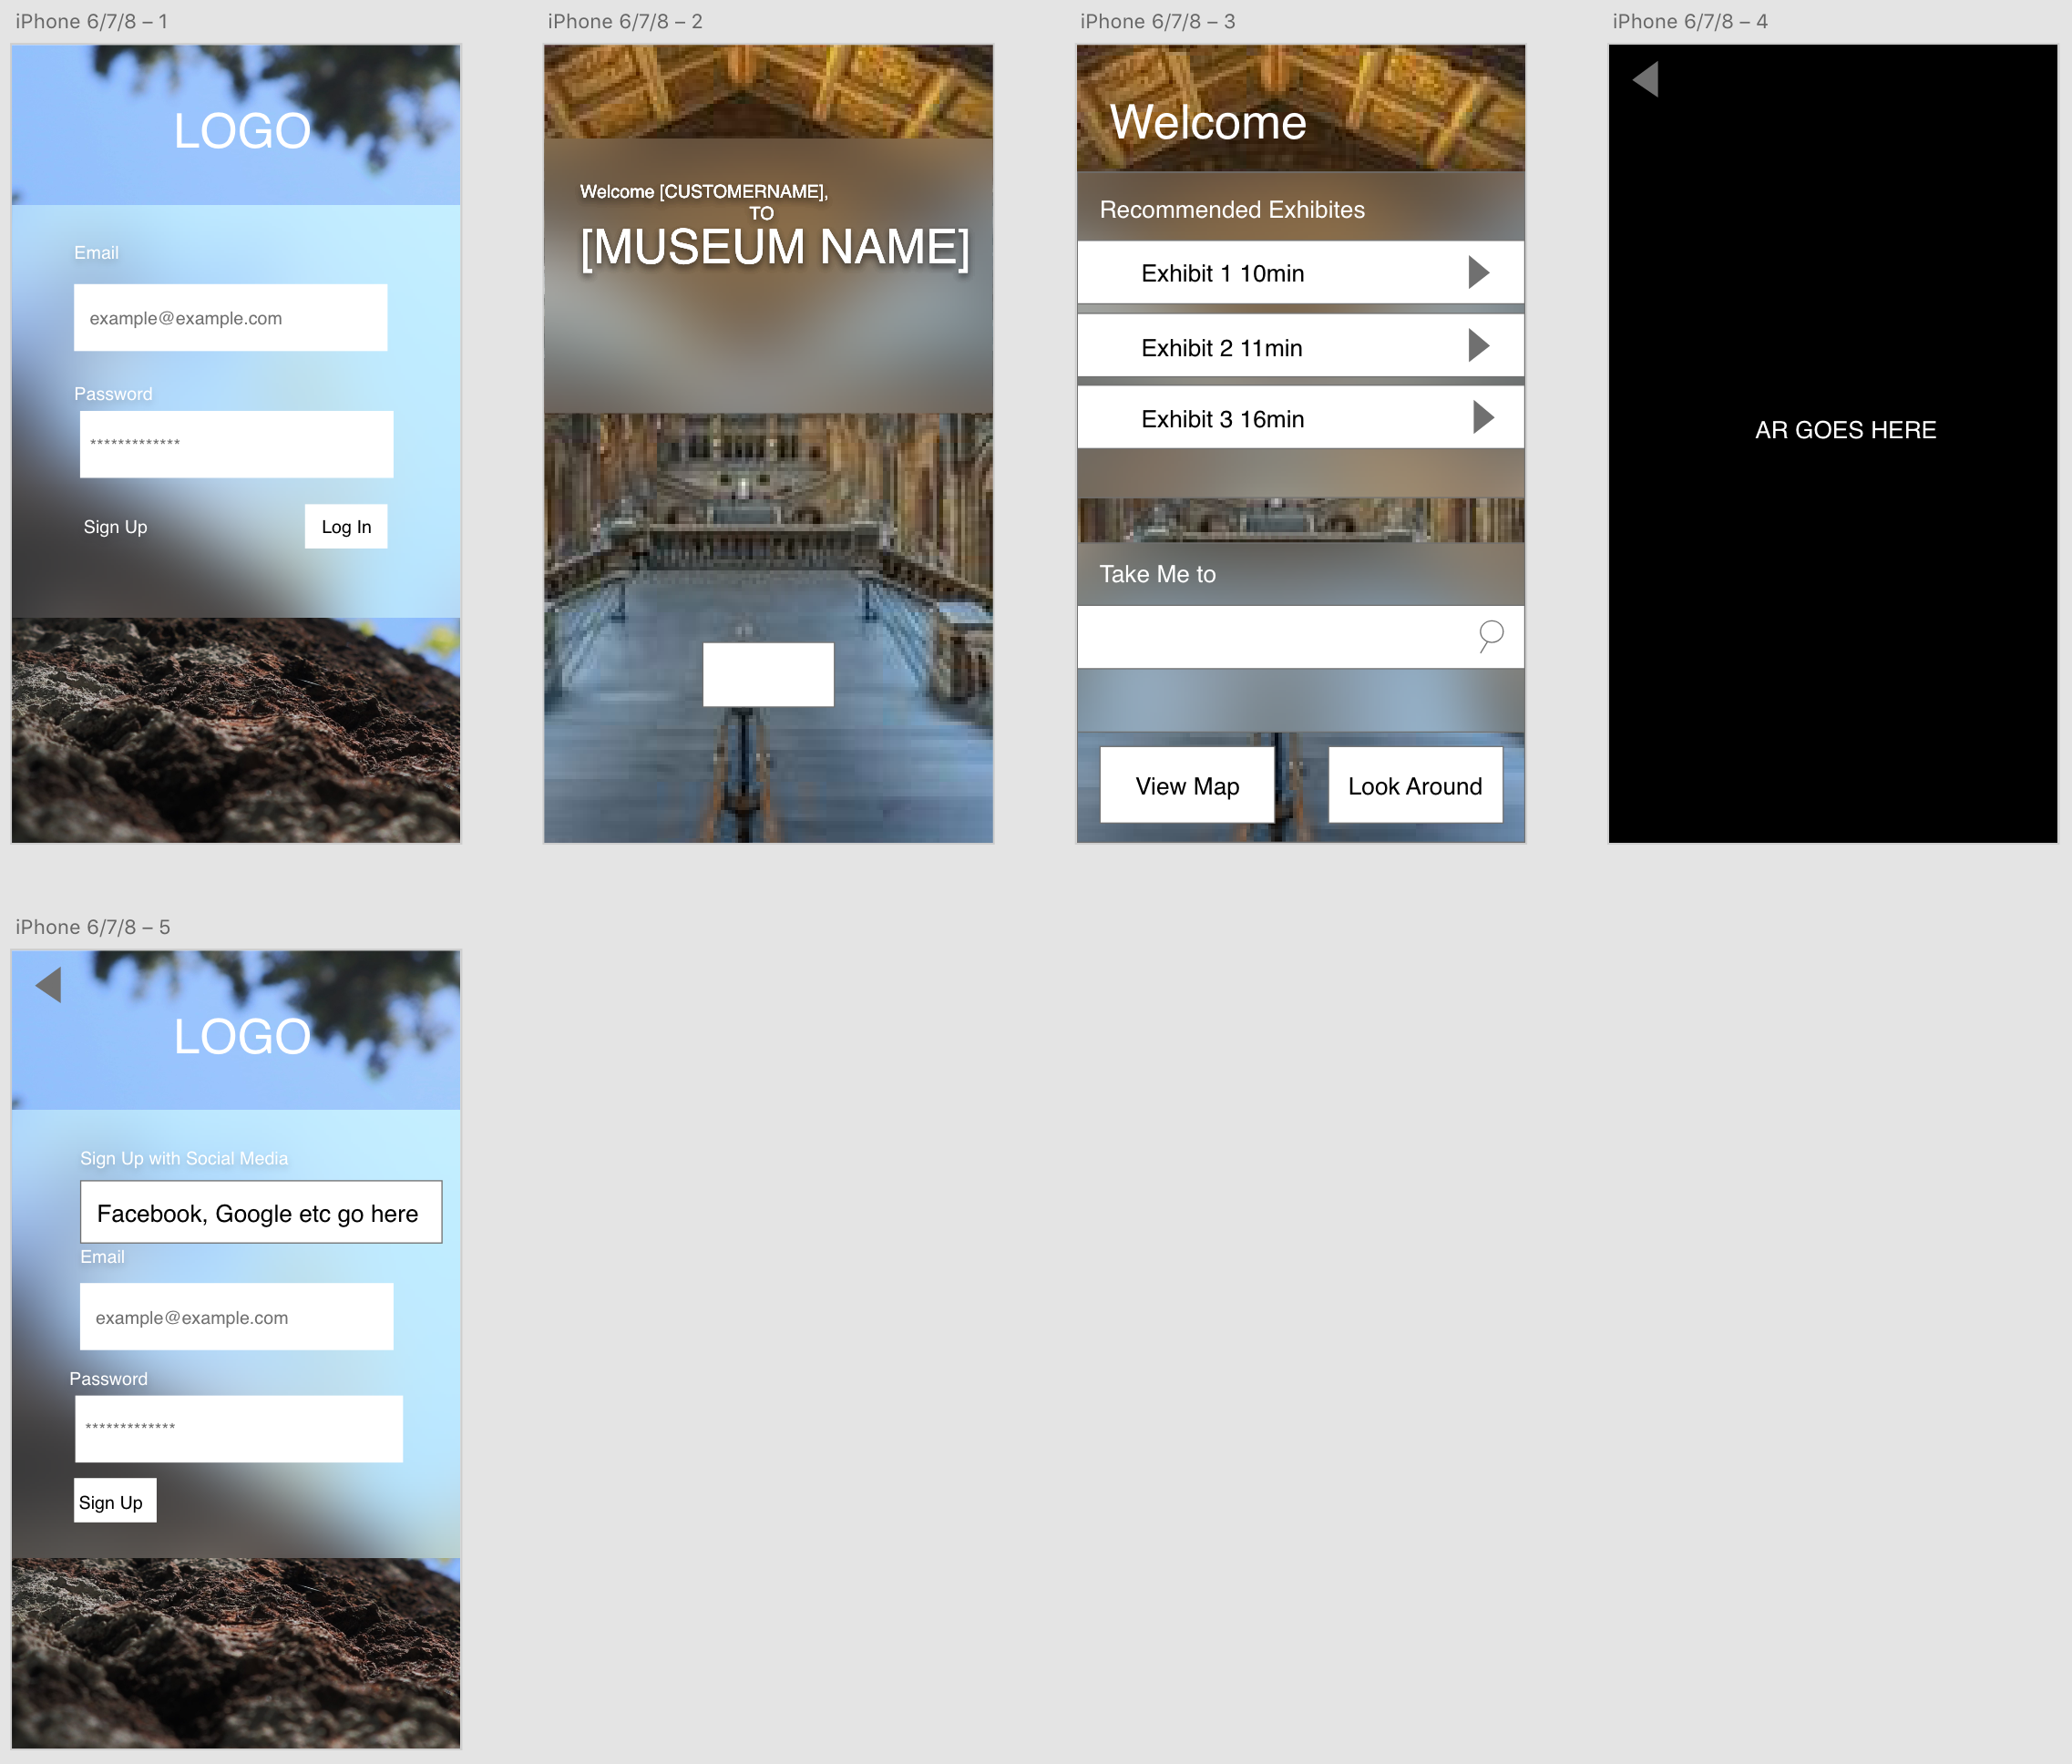
\includegraphics[width=60mm, height=100mm]{prototypes/ar/ios/3.png} }\\
\multicolumn{2}{c}{(c) Image scanned before; showing the green tick}
\end{tabular}
\caption{ARKit prototyping on iOS device}
\label{fig:ARKit}
\end{figure}


\newpage
\subsubsection{ARCore}
\begin{figure}[H]
\centering  
\begin{tabular}{cc}
  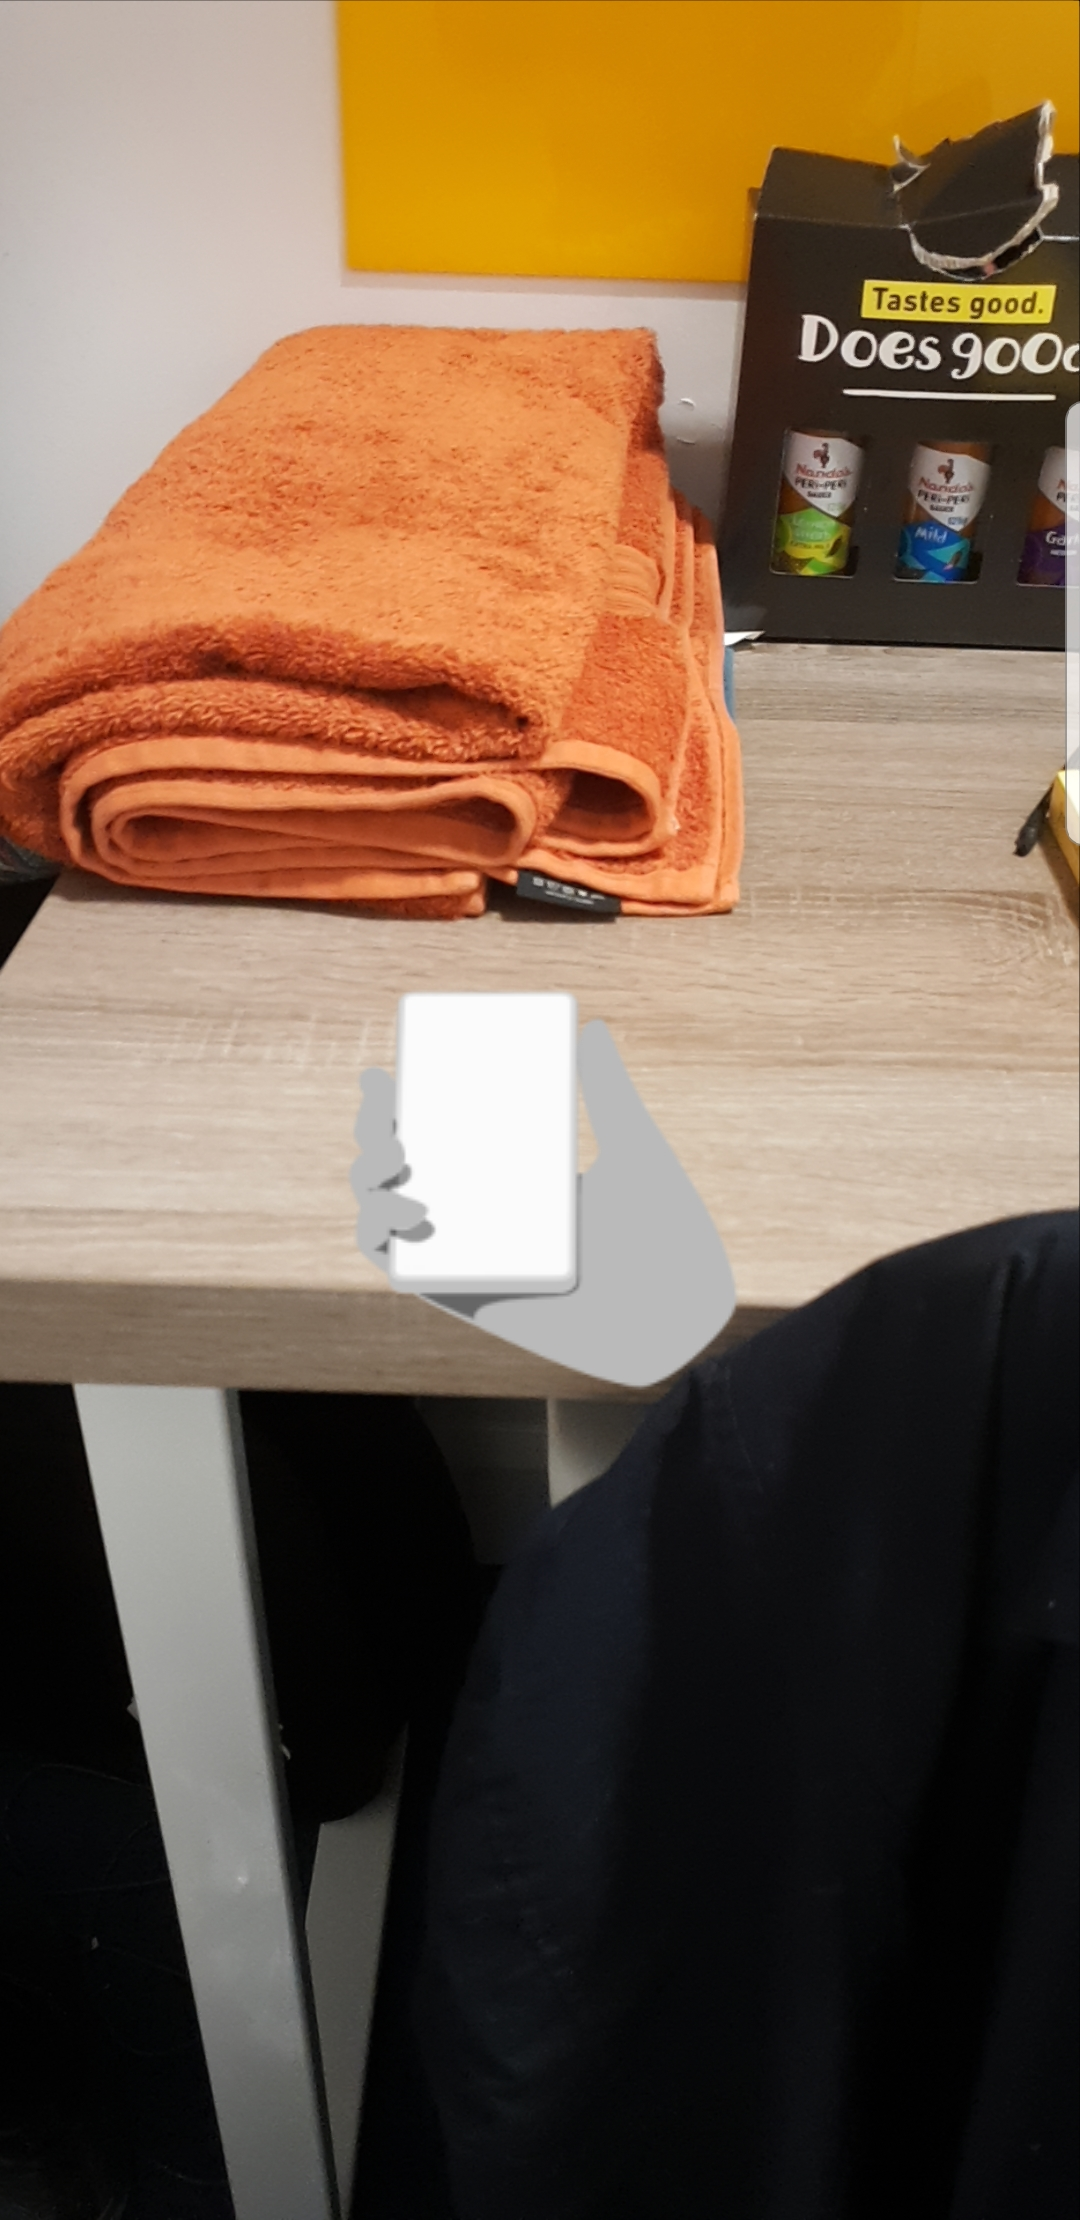
\includegraphics[width=60mm, height=100mm]{prototypes/ar/android/1.jpg} &   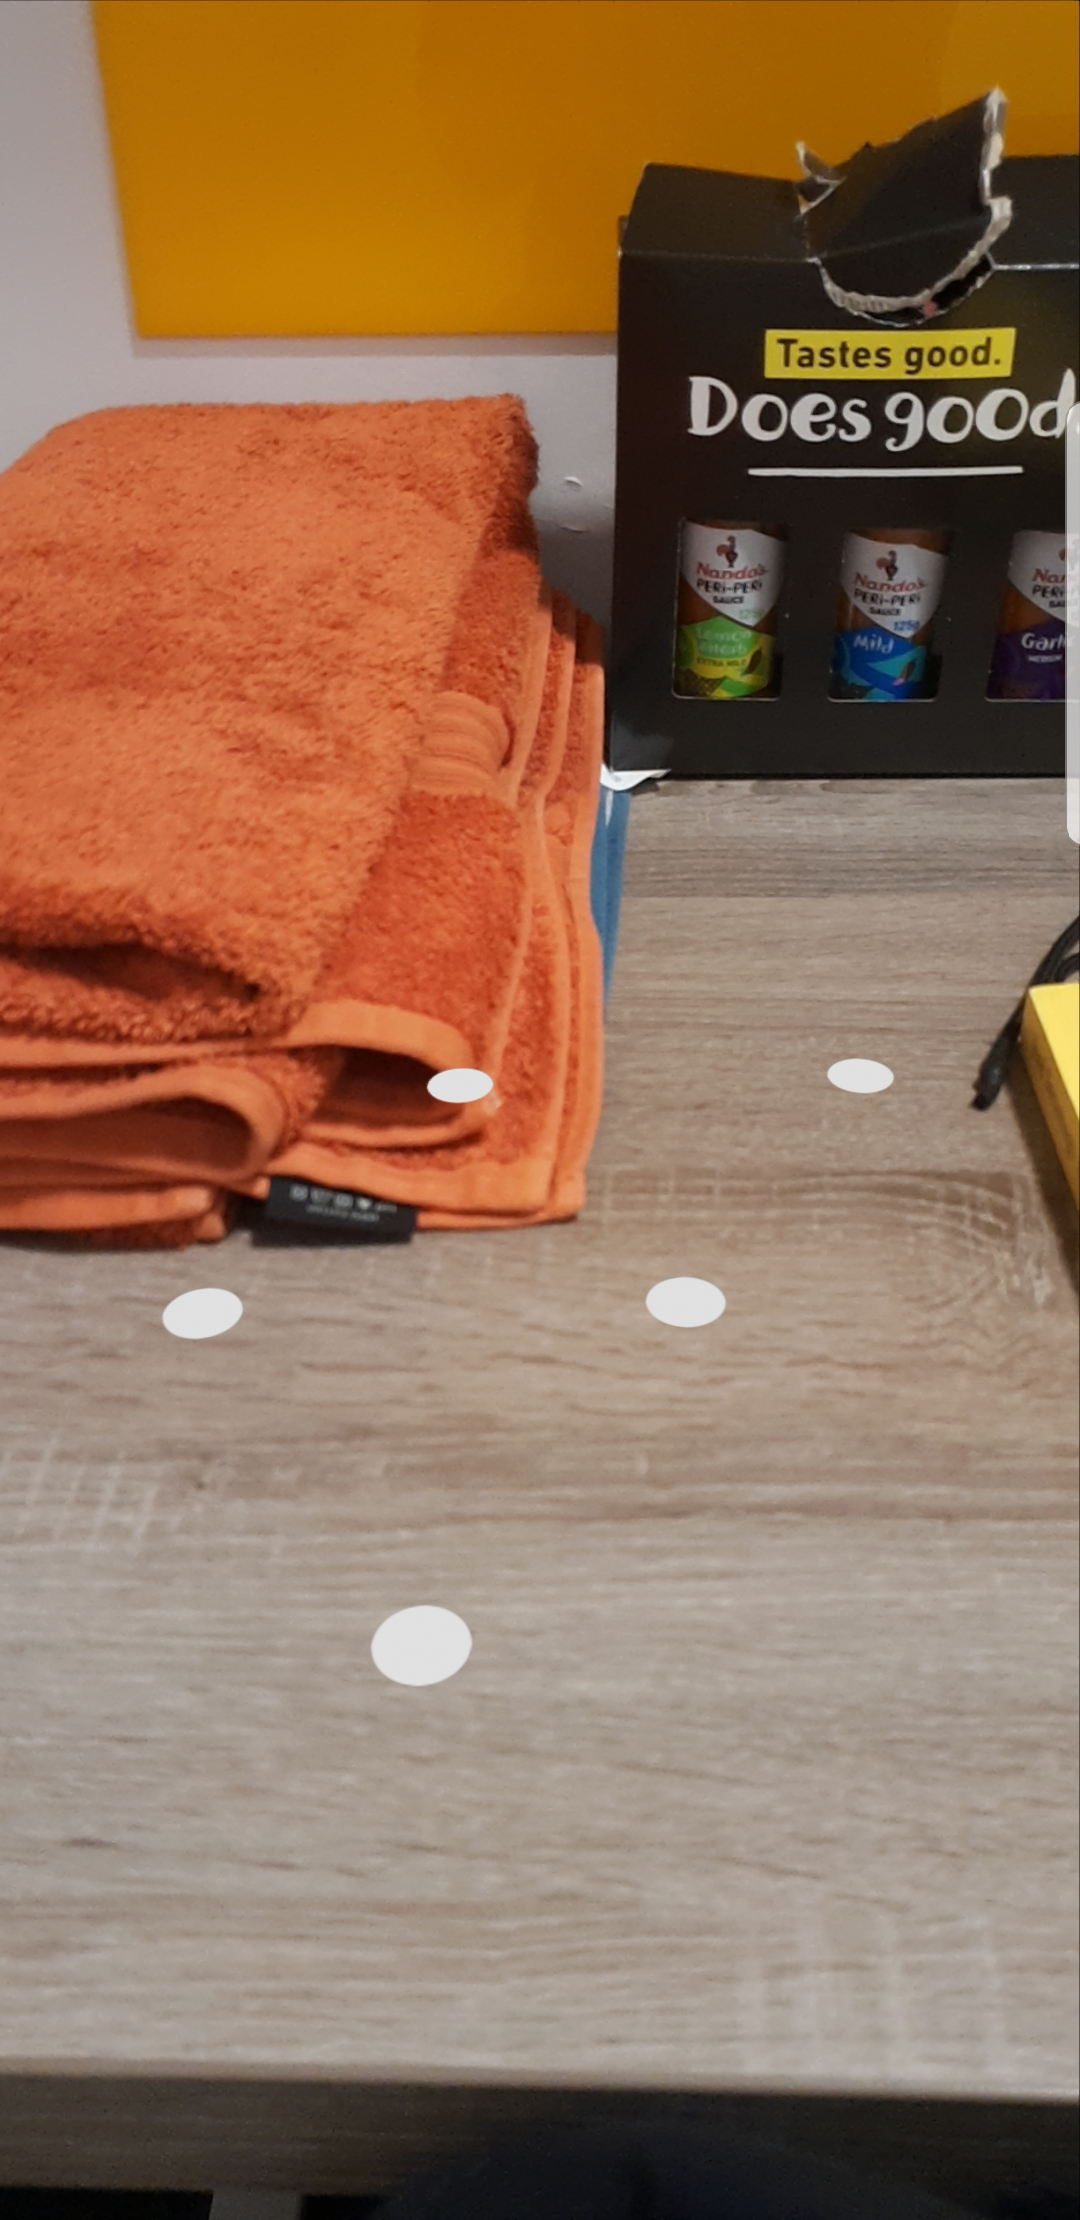
\includegraphics[width=60mm, height=100mm]{prototypes/ar/android/2.jpg} \\
(a) Initial view & (b) Detection of surface \\[6pt]
\multicolumn{2}{c}{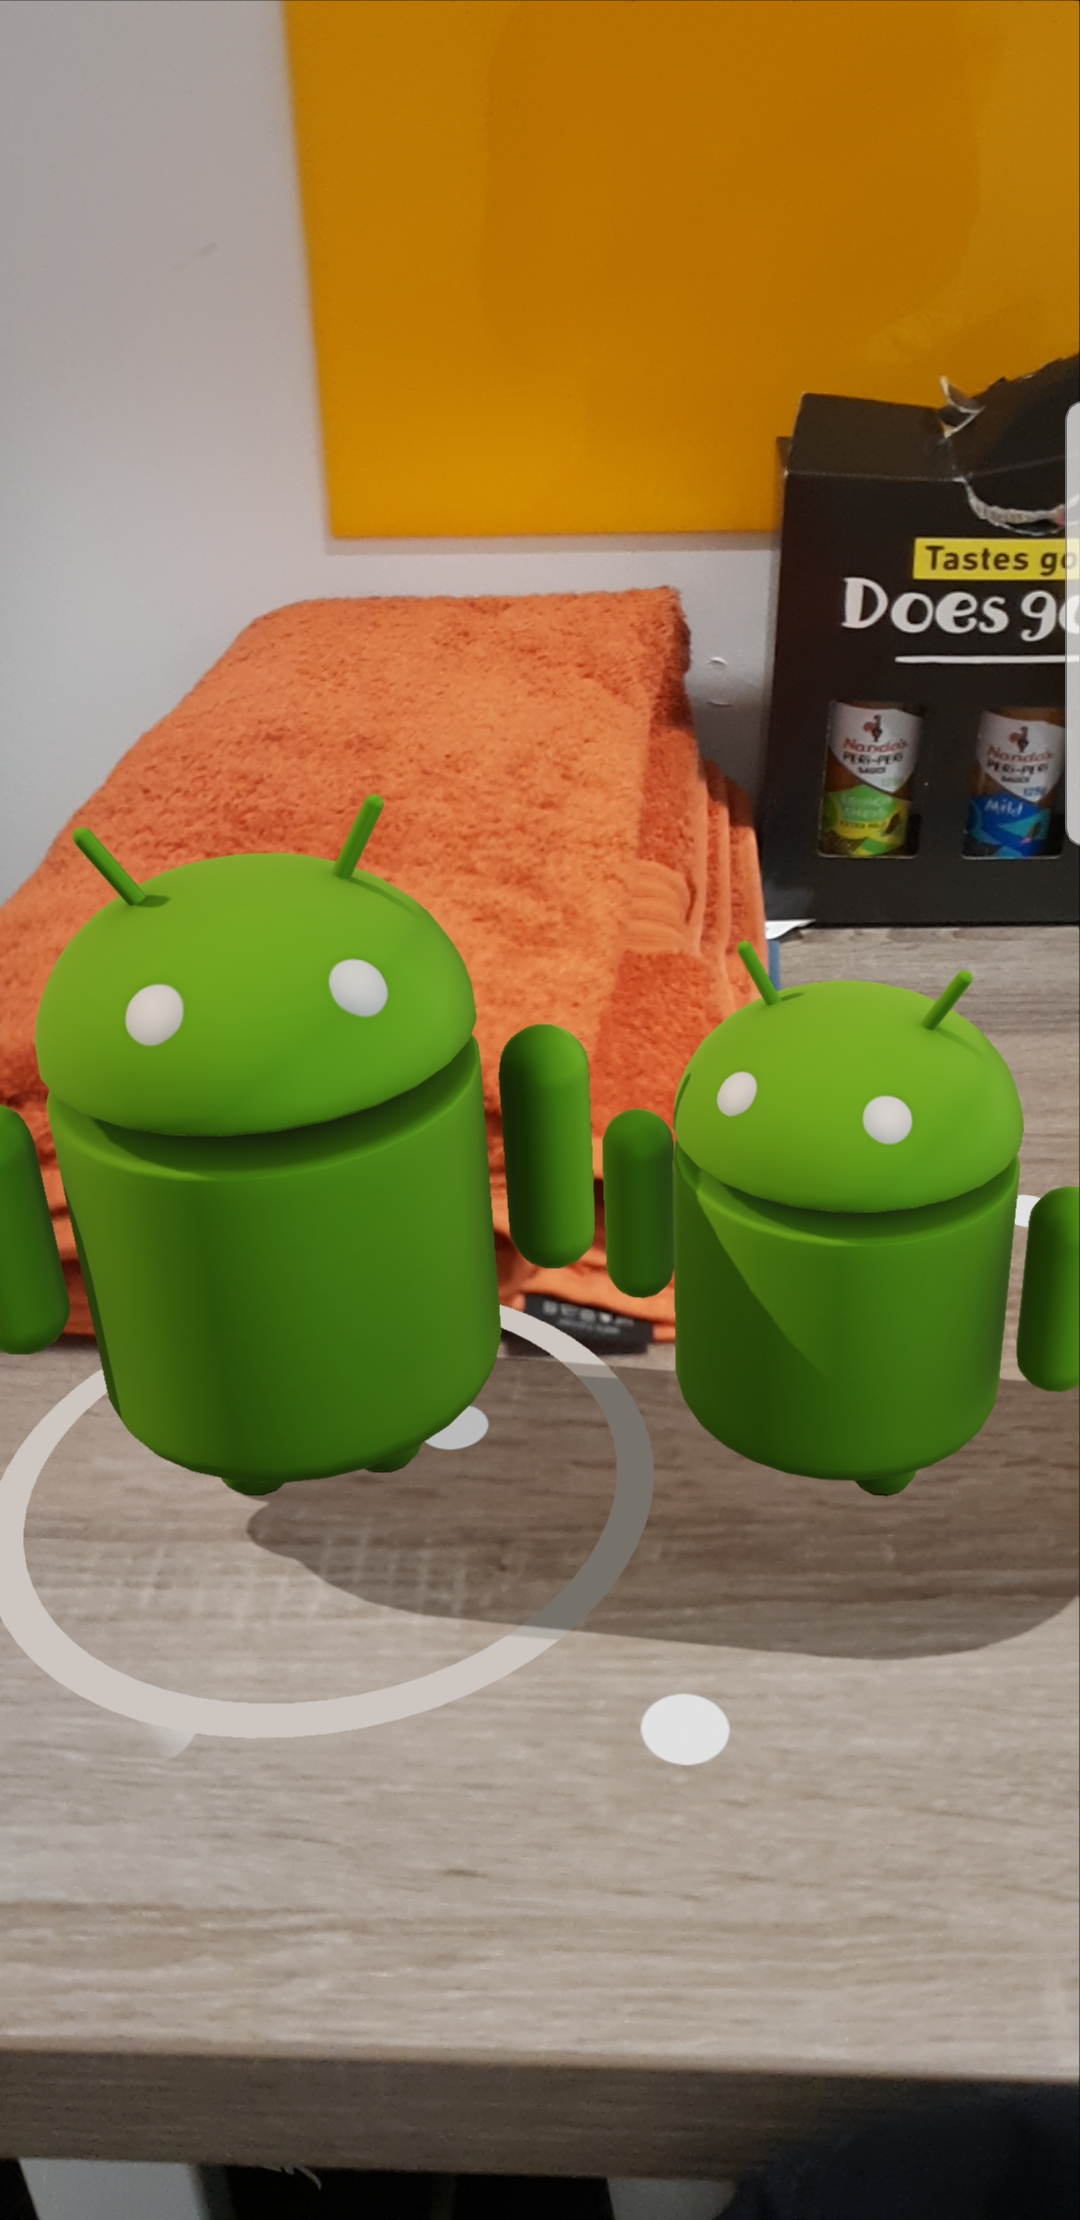
\includegraphics[width=60mm, height=100mm]{prototypes/ar/android/3.jpg} }\\
\multicolumn{2}{c}{(c) Objects superimposed on surface}
\end{tabular}
\caption{ARCore prototyping on Android device}
\label{fig:ARCore}
\end{figure}


\section{Hardware - Arduino and Raspberry Pis}
